%%%%%%%%%%%%%%%%%%%%%%%%%%%%%%%%%%%%%%%%%%%%%%%%%%%%%%%%%%%%%%%%%%%%%%%%%%%

\documentclass{standalone}

\usepackage{amsmath}
\usepackage{mathptmx}
\usepackage{pgfplots}
\usetikzlibrary{external}
\tikzexternalize{bamboo-log}
\pgfplotsset{compat=1.16}

%% IEEE uses Times Roman font, so we'll default to Times.
%% These three commands make up the entire times.sty package.
\renewcommand{\rmdefault}{ptm}
\renewcommand{\ttdefault}{pcr}
\normalfont\selectfont

\begin{document}

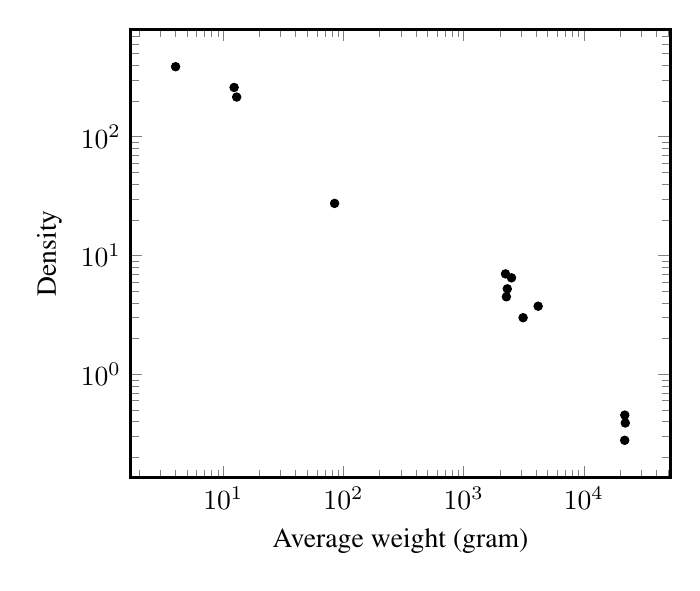
\begin{tikzpicture}
\tikzset{%%
  every mark/.append style={scale=1.0},%%
  scale=1.0%%
}
\pgfplotsset{%%
  every axis/.append style={font=\normalsize}%%
}
%%
\begin{loglogaxis}[%%
  axis line style=very thick,%%
  dotStyle/.style={mark size=1.5,black,mark color=black,mark=*,only marks},%%
  enlargelimits=true,%%
  %% x axis
  xlabel={\normalsize Average weight~(gram)},%%
  %% y axis
  ylabel={\normalsize Density}%%
]
%%
%%
\addplot[dotStyle] coordinates {
  (3122.33333333333,3)
  (4166.93333333333,3.75)
  (2267.11111111111,4.5)
  (2306.28571428571,5.25)
  (2228.69763465375,7.018)
  (21872.3098995696,0.2788)
  (22125.641025641,0.39)
  (21903.1903190319,0.4545)
  (2500.46153846153,6.5)
  (4.01028277633,389)
  (12.30769230768,260)
  (12.91666666665,216)
  (84.36363636361,27.5)
};
\end{loglogaxis}
\end{tikzpicture}

\end{document}
